\chapter{Experimental Setup and Verification}\label{ch:setup}

The numbers in Chapter~\ref{ch:results} are only as good as the code and
protocol behind them. This chapter describes the data, the baselines and how
every model was trained and evaluated, and then the tests we ran before
committing GPU time to long training runs.

\section{Dataset and Data Pipeline}\label{sec:data}

All experiments use DIV2K \cite{agustsson2017div2k}, which provides 800
high-resolution training images and 100 validation images. Training uses only
the training split; the 100 validation images are used for every result we
report. Because we did not hold out a separate test set, the reported numbers
are validation results, a limitation we return to in
Chapter~\ref{ch:conclusion}.

Our first data loader decoded a full-resolution PNG for every crop, and
training ran at roughly 1.8 steps per second because the GPU waited on the
CPU. We replaced it with a cache of 32 fixed $128\times128$ crops from each
training image, 25,600 tiles in all, stored as a single 1.26\,GB array of
8-bit pixels and memory-mapped at training time. Random flips and
90-degree rotations augment the cached crops. The degradation of
Section~\ref{sec:degradation} is still applied on the fly by four loader
workers, so every epoch sees freshly sampled blur, scale, noise and JPEG
settings. In effect the set of degraded pairs is unlimited, while the set of
clean crops is fixed (Figure~\ref{fig:pipeline}).

\begin{figure}[htbp]
	\centering
	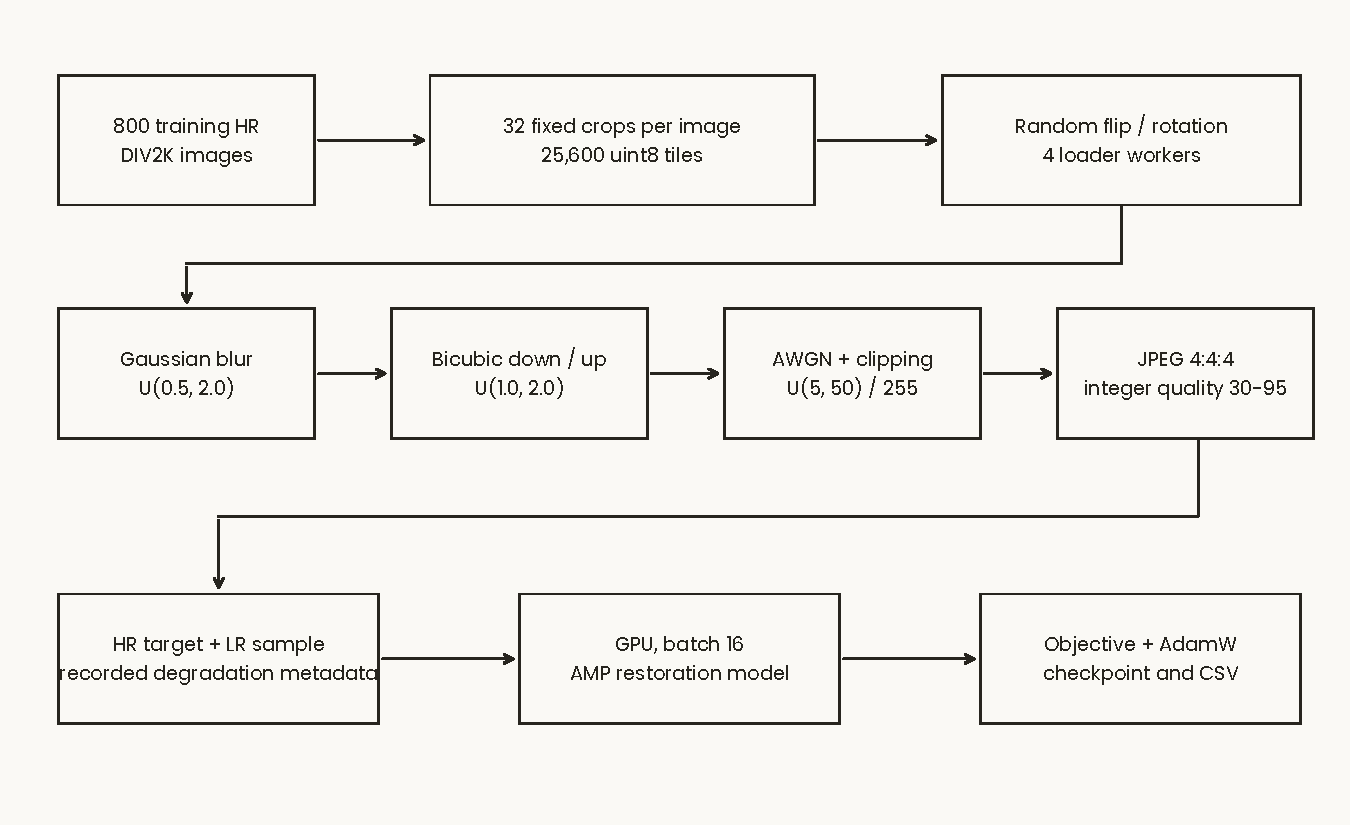
\includegraphics[width=\linewidth]{pipeline.pdf}
	\caption{Training data pipeline. Loader workers sample degradation
	parameters for each augmented clean crop and return the degraded input, the
	clean target and the parameters.}
	\label{fig:pipeline}
\end{figure}

Online degradation is good for training but awkward for anyone trying to
reproduce exact inputs. We therefore also exported a fixed set of 5,000
degraded and clean pairs generated with seed 1234, together with a manifest of
their parameters. The degradation code reproduces this set byte for byte, and
a single CPU worker generates about 233 samples per second.

\section{Baselines}\label{sec:baselines}

\paragraph{DnCNN.} Our RGB DnCNN has 17 convolutional layers of width 64
with batch normalisation and predicts the residual, giving 558,403
parameters.

\paragraph{FFDNet.} Our FFDNet follows the author's colour architecture
\cite{kair}: pixel unshuffle, 12 convolutional layers of width 96 and a
noise-level map concatenated to the input, giving 852,108 parameters. On our
composite task the noise map is a problem, because there is more to the
degradation than Gaussian noise. We therefore train two variants.
\emph{Oracle} FFDNet receives the true sampled noise level $\sigma_n$ as its
map. This is information no real user would have, so the oracle variant is an
upper reference rather than a fair competitor. \emph{Blind} FFDNet receives
a constant map of $27.5/255$, the middle of the noise range, during both
training and evaluation. It sees exactly what DnCNN and \fcsg{} see.

All four models are trained from scratch on the same composite degradation.
We do not compare against numbers published for other tasks or datasets.

\section{Training Protocol}\label{sec:training}

Every model is trained with the same configuration (Table~\ref{tab:hparams}),
differing only in the model and, for FFDNet, the noise map. The original plan
called for 300,000 updates; we reduced this to 200,000 to fit the weekly GPU
quota available to us.

\begin{table}[htbp]
	\centering
	\caption{Training configuration, identical for every method.}
	\label{tab:hparams}
	\small
	\begin{tabular}{@{}ll@{}}
		\toprule
		Setting & Value \\
		\midrule
		Optimiser            & AdamW \cite{loshchilov2019adamw}, weight decay 0 \\
		Learning rate        & $2\times10^{-4}$, cosine decay \cite{loshchilov2017sgdr} to $10^{-6}$ \\
		Updates              & 200,000 \\
		Batch                & 16 crops of $128\times128$ RGB \\
		Loss                 & $\mathcal{L}_\text{char} + 0.05\,\mathcal{L}_\text{freq}$, plus entropy term for \fcsg{} \\
		Entropy coefficient  & 0.01, linear decay to 0 (\fcsg{} only) \\
		Precision            & FP16 mixed precision \cite{micikevicius2018amp} with gradient scaling \\
		Validation           & 16 fixed crops every 2,000 updates \\
		Checkpoints          & every 2,000 updates (model, optimiser, scaler, step) \\
		Hardware             & NVIDIA Tesla T4 (Kaggle) \\
		\bottomrule
	\end{tabular}
\end{table}

Training ran in Kaggle notebook sessions, which stop after twelve hours.
Each run therefore resumes from its newest checkpoint at start-up. Checkpoints
store the model, optimiser, gradient scaler, step and configuration. They do
not store random number generator or sampler state, so a resumed run is not
bit-identical to an uninterrupted one. Training seeds were not fixed, and
each model was trained once. Recorded training-loop time was 10.06 hours for
\fcsg{}, 6.66 for DnCNN, 2.04 for blind FFDNet and 2.33 for oracle FFDNet.
Figure~\ref{fig:schedules} shows the learning-rate and entropy schedules.

\begin{figure}[htbp]
	\centering
	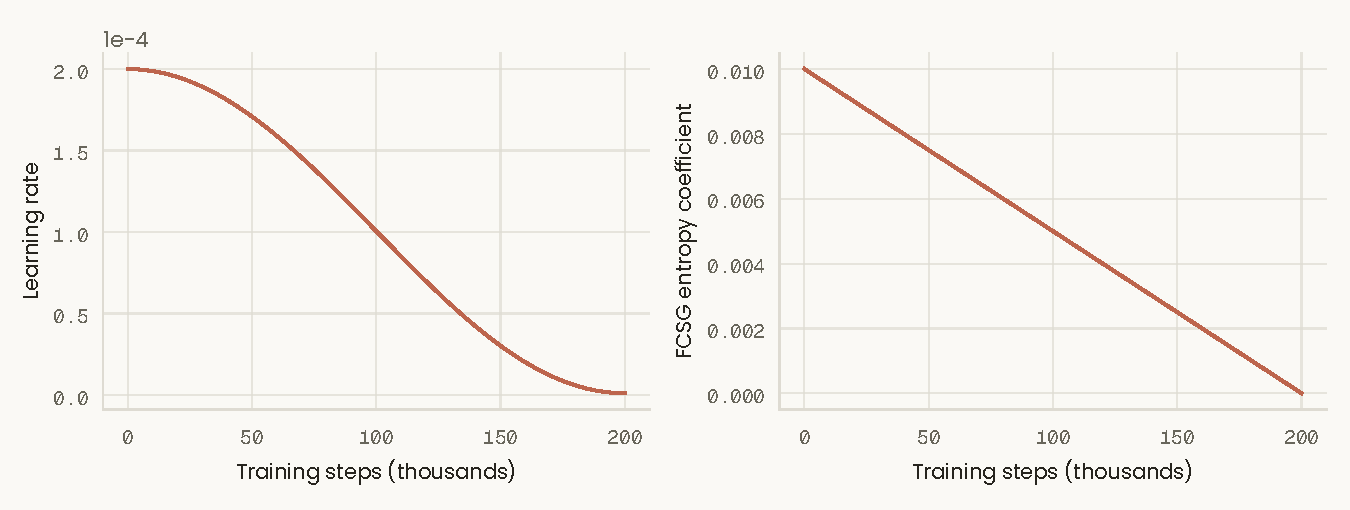
\includegraphics[width=0.85\linewidth]{schedules.pdf}
	\caption{Learning-rate and entropy-coefficient schedules over 200,000 updates.}
	\label{fig:schedules}
\end{figure}

\section{Evaluation Protocol}\label{sec:evalproto}

Final results use all 100 DIV2K validation images. Each image is degraded
once with a seed equal to its index, so every model sees exactly the same
degraded inputs. Inference is tiled: $256\times256$ tiles with 32 pixels of
overlap (stride 224), with the last tile in each direction aligned to the
image border and overlapping outputs averaged uniformly. Tiling keeps memory
low on large images; Section~\ref{sec:latency} measures how much it costs in
accuracy. Restored values are clipped to $[0,1]$ before computing PSNR, SSIM
and LPIPS as described in Section~\ref{sec:lit-metrics}.

During training we monitored a different quantity: PSNR on 16 fixed
$128\times128$ validation crops. The two are not comparable. For \fcsg{} the
final crop PSNR is 30.59\dB{} while the full-image result is 27.24\dB{}.
Crop numbers are used only for convergence curves.

\section{Implementation Verification}\label{sec:verification}

Before any long training run we ran a fixed set of checks in a single
notebook on the same Kaggle T4 (Python 3.12, PyTorch 2.10 \cite{paszke2019pytorch},
CUDA 12.8). The notebook stops at the first failure. Table~\ref{tab:gates}
lists the checks and their measured values.

\begin{table}[htbp]
	\centering
	\caption{Pre-training verification checks (Tesla T4, 25 September 2026 run).}
	\small
	\label{tab:gates}
	\begin{tabular}{@{}lll@{}}
		\toprule
		Check & Criterion & Measured \\
		\midrule
		FFDNet weights, CBSD68 $\sigma{=}25$ & within 0.5\dB{} of 31.21 & 31.220\dB \\
		Band reconstruction & $x_L{+}x_M{+}x_H = x$ & max error $6.0\times10^{-7}$ \\
		Frequency units & same band at 128 and 256 px & passed \\
		Parameter budget & $< 5$M & 97,088 \\
		Compute budget & $< 10$ GFLOPs at $256^2$ & 9.39 \\
		Memory, forward + backward & $< 4$ GB & 0.60 GB \\
		Shapes, gradients, odd sizes (AMP) & no errors & passed \\
		One-image overfit, 200 steps & MSE $<0.01$, $<\frac14$ initial & ratio 0.18 \\
		Checkpoint restore & identical outputs & passed \\
		Degradation reproducibility & byte-identical & passed \\
		\bottomrule
	\end{tabular}
\end{table}

Two of these checks deserve a word. The band reconstruction assertion is a
single line, yet it catches nearly every sign, shift and normalisation bug an
FFT implementation can have. The overfit test asks the full model to memorise
one image in 200 steps. A model that cannot do this has a bug, and finding
that out in a few seconds is far cheaper than finding it after ten hours of
training. \fcsg{} reduced the MSE from 0.0261 to 0.0046
(Figure~\ref{fig:overfit}). The memory figure was measured at batch size 1
and does not describe peak memory at the training batch size.

\begin{figure}[htbp]
	\centering
	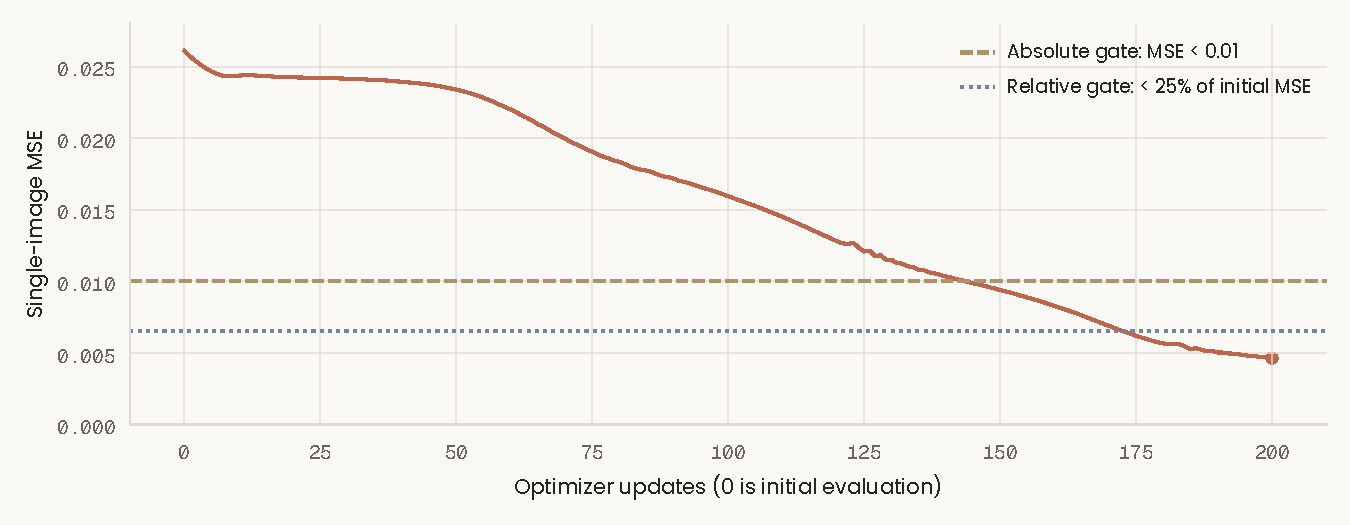
\includegraphics[width=0.75\linewidth]{overfit.pdf}
	\caption{Single-image overfit test: MSE over 200 updates.}
	\label{fig:overfit}
\end{figure}

\section{Baseline Reproduction}\label{sec:baseline-repro}

\paragraph{FFDNet.} To check our FFDNet implementation and evaluation code
against a published number, we loaded the author's pretrained colour weights
\cite{kair} and evaluated them on all 68 CBSD68 images
\cite{martin2001bsd} with unclipped Gaussian noise at $\sigma=25$, following
the author's protocol. We obtained 31.220\dB{}, against 31.21\dB{} in the
paper \cite{zhang2018ffdnet}, a difference of 0.01\dB{}. This verifies the
architecture, weight loading and evaluation path. It does not reproduce
FFDNet's training, which is why all composite models are trained from
scratch.

\paragraph{DnCNN.} As an end-to-end test of our training loop we trained
DnCNN on clipped Gaussian noise at $\sigma=25$ before moving to the composite
task. At checkpoint 286,000 it reached 32.65\dB{} on DIV2K validation and
31.04\dB{} on CBSD68 (Table~\ref{tab:gaussian}). These figures use clipped
noise and are not directly comparable with the unclipped protocol of the
FFDNet paper; they confirm that the training and evaluation code work on a
problem with a known order of magnitude.

\begin{table}[htbp]
	\centering
	\caption{DnCNN on clipped Gaussian noise, $\sigma=25$, checkpoint 286,000.}
	\label{tab:gaussian}
	\begin{tabular}{@{}lrrr@{}}
		\toprule
		Dataset & Images & Input PSNR & Output PSNR \\
		\midrule
		CBSD68           & 68  & 20.53\dB & 31.04\dB \\
		DIV2K validation & 100 & 20.70\dB & 32.65\dB \\
		\bottomrule
	\end{tabular}
\end{table}
